%
%===============>>  ГРУППА 9-2 МОДУЛЬ 4  <<=============
%
\setmodule{4}
%
%===============>>  Занятие 1  <<===============
%
%\begin{class}[number=1]
%	\begin{listofex}
%		%		В ДЗ №1
%		%		\item Вычислить рациональным способом:
%		%		\begin{enumcols}[itemcolumns=3]
%		%			\item \( \sqrt{16+4\cdot4\cdot24} \)
%		%			\item \( \sqrt{83^3\cdot2^2-83^2\cdot2^3} \)
%		%			\item \( \sqrt{50^2-4\cdot7\cdot7} \)
%		%		\end{enumcols}
%		\item Построить график функции \( y=2x-5 \).
%		\begin{enumcols}[itemcolumns=1]
%			\item Принадлежит ли точка с координатами \( (112;217) \) графику этой функции?
%			\item Найти точку пересечения графика данной функции с графиком функции \( y=4x-1 \).
%		\end{enumcols}
%		\item Построить графики функций \( f(x)=x^2-2x+1 \) и \( g(x)=x^2+6x+8 \).\\
%		Выберите верные утверждения:
%		\begin{enumcols}[itemcolumns=4]
%			\item \( f(-1)>f(1) \);
%			\item \( g(-1)<f(-1) \);
%			\item \( g(-2)=f(1) \);
%			\item \( f(3)<g(-5) \);
%		\end{enumcols}
%		\begin{enumcols}[itemcolumns=1, resume]
%			\item график функции \( f(x) \) возрастает на промежутке \( [0;+\infty) \);
%			\item график функции \( g(x) \) убывает на промежутке \( [-9;-4] \);
%			\item промежуток возрастания функции \( f(x) \) входит в промежуток возрастания функции \( g(x) \);
%			\item \( f(x)=4 \) при \( x=3 \);
%			\item наименьшее значение функция \( f(x) \) принимает в \( x=-1 \);
%			\item наименьшее значение \( f(x) \) меньше наименьшего значения \( g(x) \);
%			\item корнем уравнения \( f(x)=9 \) является только \( x=-2 \);
%			\item \( f(x)\ge0 \) при любом \( x \);
%			\item \( g(x)\le0 \) при \( x\in[-4;-2] \);
%			\item график функции \( g(x) \) пересекается c осью \( Y \) в точке \( (0;4) \).
%		\end{enumcols}
%		\item Решить систему неравенств:
%		\begin{enumcols}[itemcolumns=2]
%			\item
%			\( \left\{
%			\begin{array}{l}
%				3(x-1)-2(2-3x)>5x-3,\\
%				8x-3(2x+5)<2(x-7).
%			\end{array}
%			\right. \)
%			\item
%			\( \left\{
%			\begin{array}{l}
%				12x-3(x-5)>2x+1,\\
%				(x-7)(x+12)\le0.
%			\end{array}
%			\right. \)
%		\end{enumcols}
%		
%		\item При каких значениях переменной выражение \( \sqrt{4x+1}+\sqrt{2-3x} \) имеет смысл?
%		\item Построить график функции \( f(x)=\sqrt{x-4}+1 \).
%		\begin{enumcols}[itemcolumns=1]
%			\item определить область определения и область значений функции;
%			\item сравнить \( f(7) \) и \( f(12) \);
%			\item вычислить \( f(x)=26 \)
%			\item существует ли \( x \), при котором \( f(x)=-1 \)? Объясните это графически и аналитически.
%		\end{enumcols}
%	\end{listofex}
%	\textbf{Дежурные задачи}
%	\begin{listofex}
%		\item Первые \( 300 \) км автомобиль ехал со скоростью \( 60 \) км/ч, следующие 300 км --- со скоростью \( 100 \) км/ч, а последние \( 300 \) км --- со скоростью \( 75 \) км/ч. Найдите среднюю скорость автомобиля на протяжении всего пути.
%		\item Велосипедист выехал с постоянной скоростью из города \( А \) в город \( В \), расстояние между которыми равно \( 60 \) км. Отдохнув, он отправился обратно в \( А \), увеличив скорость на \( 10 \) км/ч. По пути он сделал остановку на \( 3 \) часа, в
%		результате чего затратил на обратный путь столько же времени, сколько на путь из \( А \) в \( В \). Найдите скорость велосипедиста на пути из \( А \) в \( В \).
%		\item Баржа прошла по течению реки 48 км и, повернув обратно, прошла ещё 36 км, затратив на весь путь 6 часов. Найдите собственную скорость баржи, если скорость течения реки равна 5 км/ч.
%	\end{listofex}
%\end{class}
%
%===============>>  Занятие 2  <<===============
%
%\begin{class}[number=2]
%	\begin{listofex}
%		\item Из закона всемирного тяготения \( F=G\cdot\dfrac{mM}{r^2} \) выразите массу \( m \) и найдите ее величину (в килограммах), если \( F=13,4 \) H, \( r=5 \) м, \( M=5\cdot10^9 \) и гравитационная постоянная \( G=6,7\cdot10^{-11} \) \( \dfrac{\text{м}^3}{\text{кг}\cdot\text{с}^2} \).
%		\item Известно, что \( c<-1 \). расположите в порядке убывания числа \( c,\; c^2,\; \dfrac{1}{c}\).
%		\begin{enumcols}[itemcolumns=4]
%			\item \( c^2,\; c,\; \dfrac{1}{c} \)
%			\item \( c^2,\; \dfrac{1}{c},\; c \)
%			\item \( c,\; c^2,\; \dfrac{1}{c} \)
%			\item \( c,\; \dfrac{1}{c},\; c^2 \)
%		\end{enumcols}
%		\item Какое из данных чисел принадлежит отрезку \( [3;4] \)?
%		\begin{enumcols}[itemcolumns=4]
%			\item \( \dfrac{45}{19} \)
%			\item \( \dfrac{52}{19} \)
%			\item \( \dfrac{68}{19} \)
%			\item \( \dfrac{77}{19} \)
%		\end{enumcols}
%		\item Постройте графики функции \( y=4x-1 \) и \( y=\dfrac{1}{2}x+2,5 \). Графически определите точку пересечения этих графиков. Во сколько раз ордината точки пересечения больше абсциссы?
%		\item Найдите точку пересечения графиков функций \( y=12x-70 \) и \( y=6x+2 \).
%		\item Постройте график функции \( f(x)=x^2-6x+8 \). Выберите верные утверждения:
%		\begin{enumcols}[itemcolumns=1]
%			\item График функции возрастает на промежутке \( [4;+\infty) \);
%			\item График функции убывает на промежутке \( [-7;7] \);
%			\item \( f(-4)<f(4) \);
%			\item \( f(x)=5 \) при \( x=0 \);
%			\item Данная функция имеет максимальное значение при \( x=9 \);
%			\item При \( x=-2 \) значение функции больше чем при \( x=0 \);
%			\item \( f(-1)=f(3) \);
%			\item \( f(x)\ge0 \) при \( x\ge4 \);
%			\item \( f(x)\ge0 \) только при \( x\ge4 \);
%			\item Данный график функции пересекается с графиком \( y=-x-8 \) в двух точках.
%		\end{enumcols}
%		\item Подставьте вместо знака \( * \) число так, чтобы функция \( y=2x^2-3x+* \) проходила через точку с координатами \( (4;15) \).
%		\item Решить систему неравенств:
%		\[ \left\{
%		\begin{array}{l}
%			6(x+2)-4(0,5-2x)>2x-6,\\
%			9x+x(2x+5)<2(x^2-7).
%		\end{array}
%		\right. \]
%		\item При каких значениях переменной выражение \( \sqrt{12x-6}+\sqrt{4-5x} \) имеет смысл?
%		\item Построить график функции \( f(x)=\dfrac{(x-7)(x-5)^2}{x-7} \). Найти область определения и область значений данной функции.
%		\item Высота равностороннего треугольника равна \( 15\sqrt{3} \). Найдите его периметр.
%	\end{listofex}
%\end{class}
%
%===============>>  Домашняя работа 1  <<===============
%
%\begin{homework}[number=1]
%	\begin{listofex}
%		\item Пусто
%	\end{listofex}
%\end{homework}
%
%===============>>  Занятие 3  <<===============
%
%\begin{class}[number=3]
%	\begin{listofex}
%		\item Пусто
%	\end{listofex}
%\end{class}
%
%===============>>  Занятие 4  <<===============
% смещение на одно занятие с прошлого месяца
%\begin{class}[number=4]
%	\begin{listofex}
%	\item Найдите значение \( a \) по графику функции \( y=ax^2+bx+c \), изображенному на рисунке.
%	\begin{center}
%		
\includegraphics[width=0.25\textwidth]{pics/G91M4L4-1}
%	\end{center}
%	\item Найдите значение \( k \) по графику функции \( y=\dfrac{k}{x} \), изображенному на рисунке.
%	\begin{center}
%		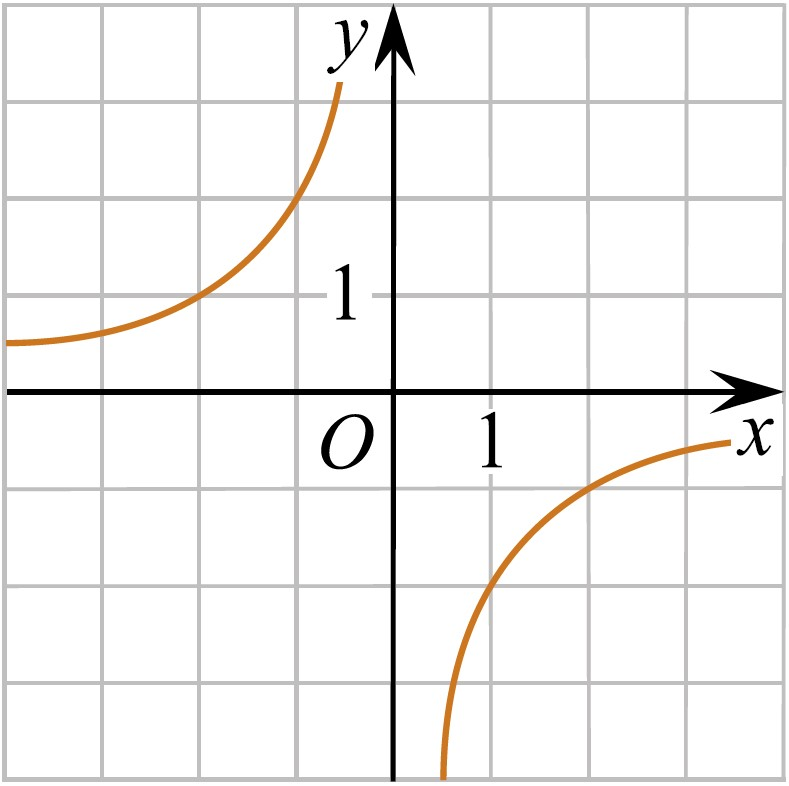
\includegraphics[width=0.25\textwidth]{pics/G91M4L4-2}
%	\end{center}
%	\begin{tasks}(4)
%		\task \( 2 \)
%		\task \( \dfrac{1}{2} \)
%		\task \( -\dfrac{1}{2} \)
%		\task \( -2 \)
%	\end{tasks}
%	\item На рисунке изображён график квадратичной функции \( y=f(x) \). Какие из следующих утверждений о данной функции неверны? Запишите их номера.
%%	\begin{center}
%%		\includegraphics[width=0.25\textwidth]{pics/G91M4L4-3}
%%	\end{center}
%	\begin{tasks}(1)
%		\task \( f(-1)=f(3) \)
%		\task Наибольшее значение функции равно \( 3 \)
%		\task \( f(x)>0 \) при \( -1<x<3 \)
%	\end{tasks}
%	
%	\item Установите соответствие между графиками функций и формулами, которые их задают.
%%	\begin{center}
%%		\includegraphics[width=0.25\textwidth]{pics/G91M4L4-3}
%%	\end{center}
%	\begin{tasks}(1)
%		\task \( y=x^2 \)
%		\task \( y=\dfrac{x}{2} \)
%		\task \( y=\sqrt{x} \)
%		\task \( y=\dfrac{2}{x} \)
%	\end{tasks}
%	\begin{center}
%		\footnotesize
%		\begin{tabular}{|c|c|c|}
%			\hline
%			А&Б&В\\
%			\hline
%			& & \\
%			\hline
%		\end{tabular}
%	\end{center}
%	
%	\item 
%	\begin{minipage}[t]{0.57\textwidth}
%		График какой из приведенных ниже функций изображен на рисунке?
%	\end{minipage}
%	\begin{minipage}[c]{0.3\textwidth}
%		
\includegraphics[align=t, width=\textwidth]{pics/G91M4L4-1}
%	\end{minipage}
%	\begin{enumcols}[itemcolumns=4]
%		\item \( y=-\dfrac{5}{x} \)
%		\item \( y=-\dfrac{1}{5x} \)
%		\item \( y=\dfrac{5}{x} \)
%		\item \( y=\dfrac{1}{5x} \)
%	\end{enumcols}
%	
%	\item 
%	\begin{minipage}[t]{0.57\textwidth}
%		Установите соответствие между функциями и их графиками.
%		\[ФУНКЦИИ\]
%		\begin{enumcols}[itemcolumns=3]
%			\item \( y=-2x+4 \)
%			\item \( y=2x-4 \)
%			\item \( y=2x+4 \)
%		\end{enumcols}
%		\[ГРАФИКИ\]	
%	\end{minipage}
%	\begin{minipage}[c]{0.3\textwidth}
%		
\includegraphics[align=t, width=\textwidth]{pics/G91M4L4-1}
%	\end{minipage}
%	\begin{center}
%		\footnotesize
%		\begin{tabular}{|c|c|c|}
%			\hline
%			А&Б&В\\
%			\hline
%			& & \\
%			\hline
%		\end{tabular}
%	\end{center}
%	
%	\item 
%	\begin{minipage}[t]{0.57\textwidth}
%		Установите соответствие между функциями и их графиками. 
%		\[ФУНКЦИИ\]
%		\begin{enumcols}[itemcolumns=3]
%			\item \( y=\dfrac{1}{9x} \)
%			\item \( y=\dfrac{9}{x} \)
%			\item \( y=-\dfrac{9}{x} \)
%		\end{enumcols}
%		\[ГРАФИКИ\]	
%	\end{minipage}
%	\begin{minipage}[c]{0.3\textwidth}
%		
\includegraphics[align=t, width=\textwidth]{pics/G91M4L4-1}
%	\end{minipage}
%	\begin{center}
%		\footnotesize
%		\begin{tabular}{|c|c|c|}
%			\hline
%			А&Б&В\\
%			\hline
%			& & \\
%			\hline
%		\end{tabular}
%	\end{center}
%	
%	\item 
%	\begin{minipage}[t]{0.57\textwidth}
%		Установите соответствие между графиками функций и формулами, которые их задают.
%	\end{minipage}
%	\begin{minipage}[c]{0.3\textwidth}
%		
\includegraphics[align=t, width=\textwidth]{pics/G91M4L4-1}
%	\end{minipage}
%	\begin{enumcols}[itemcolumns=4]
%		\item \( y=2x \)
%		\item \( y=-2x \)
%		\item \( y=x+2 \)
%		\item \( y=2 \)
%	\end{enumcols}
%	\begin{center}
%		\footnotesize
%		\begin{tabular}{|c|c|c|}
%			\hline
%			А&Б&В\\
%			\hline
%			& & \\
%			\hline
%		\end{tabular}
%	\end{center}
%	
%	\item 
%	\begin{minipage}[t]{0.57\textwidth}
%		Установите соответствие между графиками функций и формулами, которые их задают.
%	\end{minipage}
%	\begin{minipage}[c]{0.3\textwidth}
%		
\includegraphics[align=t, width=\textwidth]{pics/G91M4L4-1}
%	\end{minipage}
%	\begin{enumcols}[itemcolumns=1]
%		\item \( y=-2x^2+6x-6 \)
%		\item \( y=-2x^2-6x-6 \)
%		\item \( y=2x^2+6x+6 \)
%		\item \( y=2x^2-6x-6 \)
%	\end{enumcols}
%	\begin{center}
%		\footnotesize
%		\begin{tabular}{|c|c|c|}
%			\hline
%			А&Б&В\\
%			\hline
%			& & \\
%			\hline
%		\end{tabular}
%	\end{center}
%	
%	\item Период колебания математического маятника \( T \) (в секундах) приближенно можно вычислить по формуле \( T=2\sqrt{l} \), где \( l \) -- длина нити (в метрах). Пользуясь этой формулой, найдите длину нити маятника (в метрах), период колебаний которого составляет \( 3 \) секунды.
%	
%	\item Альпинисты в первый день восхождения поднялись на высоту \( 1400 \) м, а затем каждый следующий день поднимались на высоту на \( 100 \) м меньше, чем в предыдущий. За сколько дней они покорили высоту \( 5000 \) м?
%	
%	\item Для асфальтирования участка длиной \( 99 \) м используются \( 2  \) катка. Первый каток был установлен в одном конце участка, второй -- в противоположном. Работать они начали одновременно. Первый каток в каждую минуту проходил \( 5 \) м, а второй каток за первую минуту прошел \( 1,5 \) м, а за каждую следующую минуту проходил на \( 0,5 \) м больше, чем за предыдущую. Через сколько минут катки встретились?
%	
%	\item Занятия йогой начинают с \( 15 \) минут в день и увеличивают на \( 10 \) минут время каждый следующий день. Сколько дней следует заниматься йогой в указанном режиме, чтобы суммарная продолжительность занятий составила \( 2 \) часа?
%	
%	\item При свободном падении тело прошло в первую секунду \( 5 \) м, а в каждую следующую на \( 10 \) м больше. Найдите глубину шахты, если свободно падающее тело достигло его дна через \( 5 \) с после начала падения.
%	
%	\item Рихарду необходимо разобрать \( 315 \) квадратных уравнений. Ежедневно он разбирает на одно и то же количество уравнений больше по сравнению с предыдущем днём. Известно, что за первый день Рихард разобрал \( 11 \) квадратных уравнений, а справился со всеми он за \( 9 \) дней. Сколько уравнений Рихард разберёт в последний день?
%	
%	\item Клиент взял в банке кредит \( 100 \) рублей на n месяцев с условием, что по окончании первого месяца выплатит банку \( \dfrac{1}{n} \) часть кредита, а в каждый последующий месяц выплата будет на 5 рублей больше, чем в предыдущий. Известно, что в последний месяц выплата составила \( 55 \) руб. На какой срок был выдан кредит, если известно, что этот срок превышал полгода?
%	
%	\item 
%	\begin{minipage}[t]{0.57\textwidth}
%		При хранении бревен их укладывают, как показано на рисунке. Сколько бревен находится в одной кладке, если в ее основании положено \( 12 \) бревен?
%	\end{minipage}
%	\begin{minipage}[c]{0.3\textwidth}
%		
\includegraphics[align=t, width=\textwidth]{pics/G91M4L4-1}
%	\end{minipage}
%	
%	\item В амфитеатре 13 рядов. В первом ряду 17 мест, а в каждом следующем на 2 места больше, чем в предыдущем. Сколько всего мест в амфитеатре?
%	
%	\item 
%	\begin{minipage}[t]{0.57\textwidth}
%		Площадь ромба равна \( 54 \), а периметр равен \( 36 \). Найдите высоту ромба.
%	\end{minipage}
%	\begin{minipage}[c]{0.3\textwidth}
%		
\includegraphics[align=t, width=\textwidth]{pics/G91M4L4-1}
%	\end{minipage}
%	
%	\item 
%	\begin{minipage}[t]{0.57\textwidth}
%		Сторона ромба равна \( 4 \), а один из углов этого ромба равен \( 150\degree \). Найдите высоту этого ромба.
%	\end{minipage}
%	\begin{minipage}[c]{0.3\textwidth}
%		
\includegraphics[align=t, width=\textwidth]{pics/G91M4L4-1}
%	\end{minipage}
%	
%	\item 
%	\begin{minipage}[t]{0.57\textwidth}
%		Тангенс острого угла прямоугольной трапеции равен \( \dfrac{5}{6} \).  Найдите её большее основание, если меньшее основание равно высоте и равно \( 15 \).
%	\end{minipage}
%	\begin{minipage}[c]{0.3\textwidth}
%		
\includegraphics[align=t, width=\textwidth]{pics/G91M4L4-1}
%	\end{minipage}
%	
%	\item 
%	\begin{minipage}[t]{0.57\textwidth}
%		Основания трапеции равны \( 4 \) и \( 10 \). Найдите больший из отрезков, на которые делит среднюю линию этой трапеции одна из её диагоналей.
%	\end{minipage}
%	\begin{minipage}[c]{0.3\textwidth}
%		
\includegraphics[align=t, width=\textwidth]{pics/G91M4L4-1}
%	\end{minipage}
%\end{listofex}
%\end{class}
%
%===============>>  Домашняя работа 2  <<===============
%
\begin{homework}[number=2]
	\begin{listofex}
		\item Какое из приведенных ниже неравенств является верным при любых значениях \( a \) и \( b \), удовлетворяющих условию \( a > b \)?
		
		\textit{В ответ укажите номер правильного варианта и объясните ваш выбор.}
		\begin{tasks}(4)
			\task \( b-a < -2 \)
			\task \( a-b < -1 \)
			\task \( a-b < 3 \)
			\task \( b-a > -3 \)
		\end{tasks}
		\item \exercise{4003}
		\item Решите двойное неравенство: \( -5<\dfrac{4m-3}{3}<7 \)
		\item Решить систему неравенств:
		\begin{itasks}[2]
			\task \exercise{4029}
			\task \exercise{4031}
		\end{itasks}
		\item Футбольный мяч катится так, что за первую секунду он проходит путь \( 0,6 \) м, а в каждую следующую секунду путь увеличивается на \( 0,6  \) м по сравнению с предыдущей. Сколько секунд будет катиться мяч по горке длиной 6 метров?
		\item Основания равнобедренной трапеции равны \( 8 \) и \( 18 \), а периметр равен \( 56 \). Найдите площадь трапеции.
		\item В треугольнике \( ABC \) \( AC=3 \), \( BC=5 \), \( AB=6 \). Найдите \( \cos\angle ACB\)
		\item Задан треугольник \( ABC \). \( \sin B=0,55 \), радиус описанной около \( ABC \) окружности равен \( 5 \). Найдите \( AC \).
	\end{listofex}
\end{homework}
%
%===============>>  Занятие 5  <<===============
%
\begin{class}[number=5]
	\begin{listofex}
		\item Решить неравенство:
		\begin{tasks}(2)
			\task \( 3(2x-3)-2(3x-2)\le1-4x \)
			\task \( \dfrac{4+5x}{2}>3x+1 \)
			\task \( 36x^2-25\ge0 \)
			\task \( 9\ge\dfrac{x^2}{25} \)
			\task \( x^2-19x+18\ge0 \)
			\task \( (3x-7)^2\ge(7x-3)^2 \)
		\end{tasks}
		\item Решите двойное неравенство: \( 2x-3\le5x-2\le3-2x \)
		\item Решить систему неравенств:
		\begin{tasks}(2)
			\task
			\( \left\{
			\begin{array}{l}
				\dfrac{2x+5}{5}>\dfrac{5x+2}{2},\\[0.5em]
				\dfrac{x+2}{5}\le\dfrac{x+5}{2}.
			\end{array}
			\right. \)
			\task
			\( \left\{
			\begin{array}{l}
				x^2+9x+8\le0,\\
				-0,3x\ge2,4.
			\end{array}
			\right. \)
		\end{tasks}
		\item Решить неравенство: \( 3(\sqrt{2}-x)+\sqrt{2}(3-x)+3(3-\sqrt{2})>0 \).
		\item Решите двойное неравенство: \( 2x+3\le5x^2-9x+5\le7x+2 \).
		\item Решить систему неравенств:
		\begin{tasks}(2)
			\task
			\( \left\{
			\begin{array}{l}
				5(4x+3)-3(4x+5)\le8x+9,\\
				\dfrac{x+2}{4}+\dfrac{x+4}{2}\ge\dfrac{x+3}{5}+\dfrac{x+5}{3}.
			\end{array}
			\right. \)
			\task
			\( \left\{
			\begin{array}{l}
				2x^2-5x+2\le0,\\
				2x^2-7x+6\ge0.
			\end{array}
			\right. \)
		\end{tasks}
		\item Решить неравенство:
		\begin{tasks}(2)
			\task \( (x-2)(x-1)^2\ge0 \)
			\task \( (x^2-6x+5)(x+3)^2\le0 \)
			\task \( (3x^2-8x+4)(5x^2-8x-4)\le0 \)
			\task \( (x^2+10x+16)^2>(x^2+10x+26)^2 \)
		\end{tasks}
		\item Основания трапеции равны \( 8 \) и \( 20 \).
		
		\textit{а)} Найдите меньший из отрезков, на которые делит среднюю линию этой трапеции одна из её диагоналей.
		
		\textit{б)} Найдите отрезок средней линии, заключенный между диагоналями.
		\item Шары одинакового радиуса расположили один раз в форме правильного треугольника, а другой --- в форме прямоугольника. Найдите количество шаров, если известно, что и на стороне треугольника, и на большей стороне прямоугольника располагается на два шара больше, чем на меньшей стороне прямоугольника.
	\end{listofex}
\end{class}

%
%===============>>  Занятие 6  <<===============
%
\begin{class}[number=6]
	\begin{listofex}
		\item \( ABCDEFGH \) --- правильный восьмиугольник. Найдите угол \( EFG \).
		\item Четырёхугольник \( ABCD \) описан около окружности, \( AB=7 \), \( BC=10 \), \( CD=14 \). Найдите \( AD \).
		\item В треугольник \( ABC \) вписана окружность. В данной окружности провели три касательные так, что первая пересекает стороны \( AB \) и \( BC \), вторая --- \( AC \) и \( BC \), и третья -- \( AB \) и \( AC \). Эти касательные отсекают треугольники, периметры которых равны \( 5 \), \( 6 \), \( 7 \). Найдите периметр треугольника \( ABC \).
		\item В треугольник \( ABC \) вписана окружность, касающаяся стороны \( AB \) в точке \( M \). Пусть \( AM = x \), \( BC = a \), полупериметр треугольника равен \( p \). Докажите, что \( x = p - a \).
		\item В треугольник со сторонами \( 6 \), \( 10 \) и \( 12 \) вписана окружность. К окружности проведена касательная так, что
		она пересекает две б\textit{о}льшие стороны. Найдите периметр отсеченного треугольника.
		\item В треугольнике \( ABC \) известно, что \( AB=8 \), \( BC=10 \), \( AC=12 \). Найдите \( \cos \angle ABC \).
		\item Найдите радиус окружности, описанной около треугольника со сторонами \( 13 \), \( 14 \), \( 15 \).
		\item Стороны треугольника равны \( 1 \) и \( 2 \), а угол между
		ними равен \( 60\degree \). Через центр вписанной окружности этого треугольника и концы третьей стороны проведена окружность.
		Найдите ее радиус.
		\item В равнобедренном треугольнике с боковой стороной,
		равной \( 4 \), проведена медиана к боковой стороне. Найдите основание треугольника, если эта медиана равна \( 3 \).
		\item Медианы треугольника \( ABC \), проведенные из вершин \( B \) и \( C \), равны \( 6 \) и \( 9 \) и пересекаются в точке \( M \). Известно,
		что \( \angle BMC = 120\degree \). Найдите стороны треугольника.
	\end{listofex}
\end{class}

%
%===============>>  Домашняя работа 3  <<===============
%
%\begin{homework}[number=2]
%	\begin{listofex}
%
%	\end{listofex}
%\end{homework}
%\newpage
%\title{Подготовка к проверочной работе}
%\begin{listofex}
%	
%\end{listofex}

%
%===============>>  Занятие 7  <<===============
%
\begin{class}[number=7]
	\begin{listofex}
		\item Для числе \( p \), \( q \), \( r \), известно, что \( r<q<p \). Какая из разностей \( p-r \), \( p-q \), \( r-q \) отрицательна?
		
		\textit{В ответ укажите номер правильного варианта.}
		\begin{tasks}(4)
			\task \( p-r \)
			\task \( p-q \)
			\task \( r-q \)
			\task ни одна из них
		\end{tasks}
		\item Решить неравенство:
		\begin{tasks}(3)
			\task! \( 4x-2(x+1)>3(x-1)+5x-2,5(2x-1) \)
			\task \( 25x^2-9\le0 \)
			\task \( (2x-5)^2\ge(5x-2)^2 \)
			\task \( 64>\dfrac{4x^2}{81} \)
		\end{tasks}
		\item Решите двойное неравенство: \( 6x-5\le6-5x\le5-6x \).
		\item Решить неравенство:
		\begin{tasks}(3)
			\task \( (x-7)(2x+2)\ge0 \)
			\task \( (x-2)(x-1)^2\le0 \)
			\task \( (x^2-6x+5)(x+3)^2>0 \)
			\task! \( (2x-3)(x^2-x-2)\le(2x-3)(10x^2+11x+2) \)
		\end{tasks}
		\item Шары одинакового радиуса расположили один раз в форме правильного треугольника,
		а другой --- в форме прямоугольника. Найдите количество шаров,
		если известно, что и на стороне треугольника,
		и на большей стороне прямоугольника располагается на два шара больше,
		чем на меньшей стороне прямоугольника.
	\end{listofex}
\end{class}
%
%===============>>  Провечная работа  <<===============
%
\begin{exam}
	\begin{listofex}[start=6]
		\item Решите систему неравенств:
		\( \left\{
		\begin{array}{l}
			x^2+9x+8\le0,\\
			-0,3x\ge2,4.
		\end{array}
		\right. \)
		\item Площадь ромба \( S \) (в м\( ^2 \)) можно вычислить по формуле \( S=\dfrac{1}{2}d_1d_2 \), где \( d_1 \), \( d_2 \) --- диагонали ромба (в метрах). Пользуясь этой формулой, найдите диагональ \( d_1 \), если диагональ \( d_2 \) равна \( 30 \) м, а площадь ромба равна \( 120 \) м\( ^2 \).
		\item На стороне \( AC \) треугольника \( ABC \) отмечена точка \( D \) так,
		что \( AD = 4 \), \( DC = 8 \).
		Площадь треугольника \( ABC \) равна \( 36 \).
		Найдите площадь треугольника \( BCD \).
		\item Периметр треугольника равен \( 54 \), одна из сторон равна \( 15 \),
		а радиус вписанной в него окружности равен \( 1 \).
		Найдите площадь этого треугольника.
		\item Периметр ромба равен \( 32 \), а тангенс одного из углов равен \( \dfrac{5\sqrt{39}}{39} \).
		Найдите площадь ромба.
		\item Основания трапеции равны \( 18 \) и \( 12 \),
		одна из боковых сторон равна \( 6 \),
		а тангенс угла между ней и одним из оснований равен \( \dfrac{\sqrt{2}}{4} \).
		Найдите площадь трапеции.
		
		\item Найдите большую диагональ ромба, сторона которого равна \( \sqrt{3} \), а острый угол равен \( 60\degree \).
		\item Найдите косинусы углов трапеции с основаниями,
		равными \( 3 \) и \( 7 \) и боковыми сторонами, равными \( 2 \) и \( 5 \).
		\item Стороны \( AC \), \( AB \), \( BC \) треугольника \( ABC \) равны \( 2\sqrt{5} \), \( \sqrt{7} \) и \( 2 \) соответственно. Точка \( K \) расположена вне треугольника \( ABC \), причем отрезок \( KC \) пересекает сторону \( AB \) в точке, отличной от \( B \). Известно, что треугольник с вершинами \( K \), \( A \) и \( C \) подобен исходному. Найдите косинус угла \( AKC \), если \( \angle KAC>90\degree \).
	\end{listofex}
\end{exam}